%! Author = joels
%! Date = 05/01/2021

\section{Data Binding}
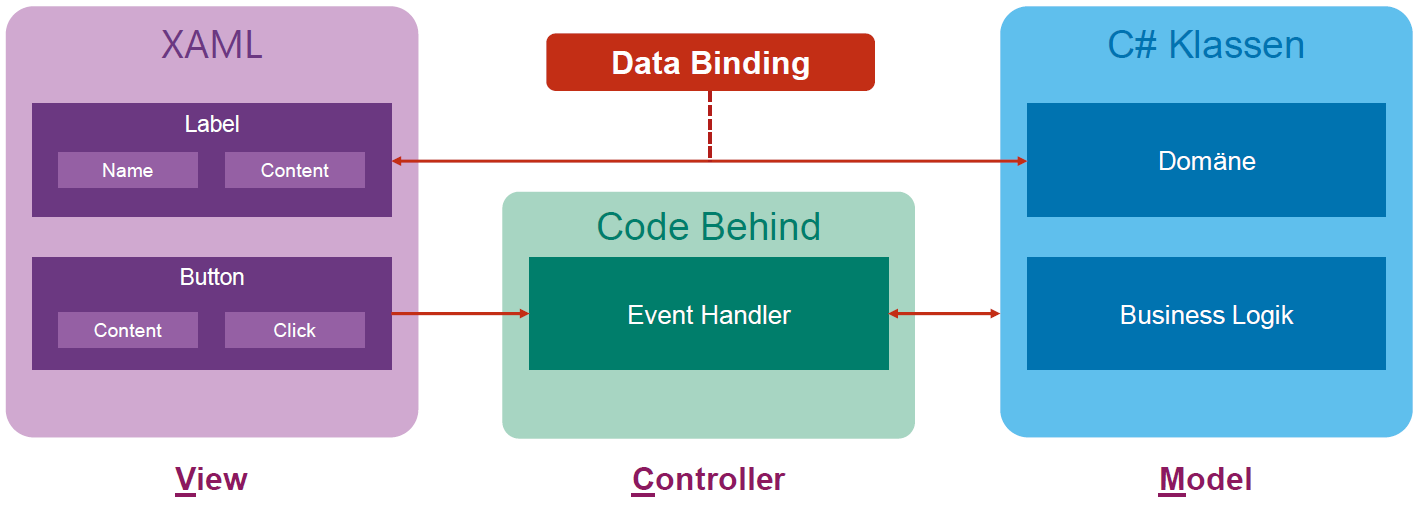
\includegraphics{data_binding_1.png}
\subsection{Data Binding in WPF}
\begin{lstlisting}
// User.cs
public class User {
    public string FirstName { get; set; } = "Joel";
    public string LastName { get; set; } = "Schaltegger";
}

// XAML
<Window>
  <StackPanel>
    // DataBinding mit Murkup Extension
    <Label Content="{Binding FirstName}" />
    <Label Content="{Binding LastName}" />
  </StackPanel>
</Window>

// Code Behind
public partial class MainWindow : Window {
    private readonly User user;
public MainWindow() {
    InitializeComponent();
    user = new User();
    this.DataContext = user; // Datenquelle für DataBinding
    }
}
\end{lstlisting}
\subsubsection{Binding Typen}
\textbf{Bindings verknüpfen Ziel und Quelle miteinander.}\\
\textcolor{blue}{Binding:} für 1:1 Verknüpfungen\\
\textcolor{blue}{MultiBinding:} für 1:n Verknüpfungen\\
\textcolor{blue}{PriorityBinding:} für 1:n / 1:1 Verknüpfungen

\subsection{Binding Typen}
\textbf{Path:} Name der Quell-Eigenschaft. Objektpfad-Syntax möglich (z.B. x.y.z)\\
\textbf{Mode:} Richtung des Datenflusses.\\
\textbf{Converter:} Datenumwandlung zwischen Quelle und Ziel.
\begin{lstlisting}
<!-- Attribute Syntax + Markup Extension -->
<TextBox Text="{Binding Path=FirstName,
    Mode=TwoWay,
    Converter={StaticResource MyCnv}}" />
<!-- Property Element Syntax -->
<TextBox>
    <TextBox.Text>
        <Binding Path="FirstName"
            Mode="TwoWay"
            Converter="{StaticResource MyCnv}" />
    </TextBox.Text>
</TextBox>
\end{lstlisting}
\subsubsection{DataBinding - Mode}
\begin{itemize}[topsep=0pt, leftmargin=4mm]
    \setlength\itemsep{-0.3em}
    \item OneTime - Einmalige Aktualisierung des Ziels beim Setzen der Quelle
    \item OneWay - Ziel wird bei Änderungen der Quelle aktualisiert
    \item OneWayToSource - Quelle wird bei Änderungen des Zieles aktualisiert
    \item TwoWay - Änderungen werden in beide Richtungen propagiert
    \item Default - Wert abhängig von Ziel-Eigenschaft
\end{itemize}
\subsubsection{DataBinding - Value Converter}
\textbf{Datenumwandlung zwischen Quelle und Ziel.} Bsp: Bool zu Visibility, Strings konvertieren. Mithilfe von \textcolor{blue}{IValueConverter}:\\
\textbf{Convert(...)} - Quelle zu Ziel. \textbf{ConvertBack(...)} - Ziel zu Quelle\\
\textbf{Erzeugung von Converter:}\\
Option1: In resources (\textcolor{blue}{StaticResource}). Option2: In Code (\textcolor{blue}{x:static})
\begin{lstlisting}
// C#
// Parameter der Methoden gekürzt zwecks Lesbarkeit
public class ReverseConverter : IValueConverter {
    public object Convert(object value, ... ) {
        var stringValue = (string) value;
        var reversedChars = stringValue.Reverse().ToArray();
        var reversedString = new string(reversedChars);
        return reversedString;
    }
    public object ConvertBack(object value, ... ) {
        return Convert(value, ... );
    }
}
\end{lstlisting}
\subsubsection{DataBinding - Weitere Eigenschaften}
\begin{itemize}[topsep=0pt, leftmargin=4mm]
    \setlength\itemsep{-0.3em}
    \item Delay - Verzögerung in Millisekunden bei Updates vom Ziel zu Quelle
    \item StringFormat - Formatangabe für Bindings mit dem Zieltyp string
    \item FallbackValue - Ergebnis, wenn Binding fehlschlägt (z.B. falscher Pfad)
    \item TargetNullValue - Ergebnis, wenn Quell-Eigenschaft null liefert
    \item UpdateSourceTrigger - Zeitpunkt, zu welchem das Quell-Element aktualisiert wird. z.B. LostFocus oder PropertyChanged; Standard abhängig vom Ziel
\end{itemize}
\subsubsection{Multi Binding}
\textbf{Verwendung analog zu Binding.} Unterschiede: Beliebig viele Quell-Eigenschaften. Nur Property Element Syntax. Converter mit IMultiValueConverter.
\begin{lstlisting}
<TextBlock>
  <TextBlock.Text>
    // { } startet das "Escaping": nachfolgende Zeichen als String interpretieren
    <MultiBinding StringFormat="{}{0} {1} ({2} Jahre)">
      <Binding Path="FirstName" />
      <Binding Path="LastName" />
      <Binding Path="Age" />
    </MultiBinding>
  </TextBlock.Text>
</TextBlock>
\end{lstlisting}
\subsubsection{Data Context}
\begin{itemize}[topsep=0pt, leftmargin=4mm]
    \setlength\itemsep{-0.3em}
    \item Property der Klasse FrameworkElement
    \item Setzt die Standardquelle für Bindings
    \item Falls undefiniert: Traversierung des Logical Trees nach oben bis zum ersten Treffer
    \item Jeder Path ist relativ zum DataContext
    \item Beliebige Objekte möglich: C\#-Klassen, WPF-Elemente, etc. Typischerweise: View Models (Woche 12)
\end{itemize}
\subsubsection{Data Context überschreiben}
\textbf{Der Data Context lässt sich für einzelne Elemente anpassen.}\\
Option1: Im Code Behind das Property \textcolor{blue}{DataContext} für das Element ersetzen. Option2: \textcolor{blue}{Source} im Binding setzen.\\
$\rightarrow$ Eher unüblich: Meist wird ein Data Context pro \textcolor{blue}{Window} verwendet.
\subsubsection{Weitere Quellen}
Mit \textcolor{blue}{RelativeSource} werden Elemente im Visual Tree referenziert:
\begin{lstlisting}
<Label Content="{Binding RelativeSource={RelativeSource FindAncestor, AncestorType=Window}, Path=Title}" />
\end{lstlisting}
Mit \textcolor{blue}{ElementName} werden Elemente über Namen referenziert:
\begin{lstlisting}
<TextBox Name="MyText" Text="Hallo MGE" />
<TextBox Text="{Binding ElementName=MyText, Path=Text}" />
\end{lstlisting}
\subsubsection{Design Time Support}
Der XAML Designer kennt den Typ des Objekts im Data Context standardmässig nicht. Das heisst: keine Autovervollständigung verfügbar (IntelliSense). Als Abhilfe kann das Attribut \textcolor{blue}{d:DataContext} beim Window gesetzt werden:
\begin{lstlisting}
// Variante 1: Objekterzeugung in XAML und Markup Extension {d:DesignInstance ... }
d:DataContext="{d:DesignInstance Type=local:User, IsDesignTimeCreatable=True}"
// Variante 2: Objekterzeugung in C# und Markup Extension {x:Static ... }
d:DataContext="{x:Static local:DesignerData.User}"
\end{lstlisting}
\subsection{Aktualisierung von Daten}
\subsubsection{POCOs als Data Context}
Als Datenquelle können beliebige Objekte verwendet werden, also auch POCOs (Plain Old CLR Objects). Unsere Bindings funktionieren – allerdings nur mit Einschränkungen. Besser: \textcolor{blue}{INotifyPropertyChanged}.
\subsubsection{INotifyPropertyChanged}
Bestandteil des .NET Framework. Ein Interface mit nur einem Event. Name des geänderten Property in \textcolor{blue}{EventArgs}.
\begin{lstlisting}
public interface INotifyPropertyChanged {
    event PropertyChangedEventHandler PropertyChanged;
}

public delegate void PropertyChangedEventHandler(object sender, PropertyChangedEventArgs eventArgs);

public class PropertyChangedEventArgs : EventArgs {
    public PropertyChangedEventArgs(string propertyName) {
        this.PropertyName = propertyName;
    }
    public virtual string PropertyName { get; }
}
\end{lstlisting}
\subsubsection{Beispiel INotifyPropertyChanged}
\textbf{\textcolor{blue}{Ohne Hilfsmittel:}}
\begin{lstlisting}
// User.cs
public class User : INotifyPropertyChanged {
  // Property mit Zugehörigem Backing Field
  private string _firstName = "Joel";
  public string FirstName {
    get => _firstName;
    set {
      if (_firstName != value) {
        _firstName = value;
        OnPropertyChanged(nameof(FirstName));
      }
    }
  }
  // Implementation von INotifyPropertyChanged
  public event PropertyChangedEventHandler PropertyChanged;
  // Event Invoker: Erzeugt Argumente und löst Event aus
  protected virtual void OnPropertyChanged(string name) {
    var eventArgs = new PropertyChangedEventArgs(name);
    PropertyChanged?.Invoke(this, eventArgs);
  }
}
\end{lstlisting}
\textbf{\textcolor{blue}{Mit Basisklasse User.cs:}}
\begin{lstlisting}
// User.cs
public class User : BindableBase {
    private string _firstName = "Joel";
    public string FirstName {
        get => _firstName;
        set => SetProperty(ref _firstName, value);
    }
}
// BindableBase.cs
public abstract class BindableBase : INotifyPropertyChanged {
  // Implementation von INotifyPropertyChanged
  public event PropertyChangedEventHandler PropertyChanged;
  // Event Invoker: Erzeugt Argumente und löst Event aus
  protected virtual void OnPropertyChanged(string name) {
    var eventArgs = new PropertyChangedEventArgs(name);
    PropertyChanged?.Invoke(this, eventArgs);
  }
  // CallMemberName wird in Namen des Property umgewandelt
  protected bool SetProperty<T>(ref T field, T value, [CallerMemberName] string name = null) {
    if (Equals(field, value)) {
      return false;
    }
    field = value;
    OnPropertyChanged(name);
    return true;
  }
}
\end{lstlisting}
\subsection{Collections}
Um eine Collection zu binden muss die Quelle \textcolor{blue}{INotifyCollectionChanged} implementieren und die Ziel-Eigenschaft eine Collection erwarten.
\subsubsection{INotifyCollectionChanged}
\textbf{Ist Bestandteil des .NET Framework.} Enthält (wie INPC) nur ein Event. Collection-Änderung wird in Event Args beschrieben. \textcolor{blue}{ObserverableCollection$<$T$>$} implementiert INPC und INCC.
\subsubsection{ItemsControl}
Wichtigste Basisklasse für WPF-Elemente zur Anzeige von Collections. Definiert folgende Ziel-Eigenschaften:
\begin{itemize}[topsep=0pt, leftmargin=4mm]
    \setlength\itemsep{-0.3em}
    \item Items – Enthält angezeigte Elemente
    \item ItemsSource – Füllt Inhalt über Data Binding ab
    \item ItemTemplate – Definiert das Template für die Darstellung eines Items
\end{itemize}
$\rightarrow$ Bei Verwendung von ItemsSource wird Items zu einer read-only Eigenschaft umgewandelt. Keine Kombination!
\begin{lstlisting}
// User.cs
public class User {
    public string FirstName { get; set; } = "Joel";
    public string LastName { get; set; } = "Schaltegger";
}

// XAML
<Window>
  <ListBox ItemsSource="{Binding}">
    <ListBox.ItemTemplate>
      <DataTemplate>
        <StackPanel>
          <TextBlock Text="{Binding LastName}"/>
          <TextBlock Text="{Binding FirstName}"/>
        </StackPanel>
      </DataTemplate>
    </ListBox.ItemTemplate>
  </ListBox>
</Window>

// Code Behind
public partial class MainWindow : Window {
    private ObservableCollection<User> users;
    public MainWindow() {
        InitializeComponent();
        // Die Collection müsste natürlich befüllt werden ..
        users = new ObservableCollection<User>();
        this.DataContext = users;
    }
}
\end{lstlisting}
\subsubsection{Item Template als Resource}
Das Item Template kann als Resource definiert werden. Das Template ist so wiederverwendbar und der XAML Code schlanker. Durch das Attribut DataType ist IntelliSense gewährleistet.
\begin{lstlisting}
<Window>
  <Window.Resources>
    <DataTemplate x:Key="UserTemplate"
        DataType="local:User">
      <StackPanel>
        <TextBlock Text="{Binding LastName}"/>
        <TextBlock Text="{Binding FirstName}"/>
      </StackPanel>
    </DataTemplate>
  </Window.Resources>
  <ListBox ItemsSource="{Binding}"
      ItemTemplate="{StaticResource UserTemplate}" />
</Window>
\end{lstlisting}
\subsubsection{Selector}
Erweitert \textcolor{blue}{ItemsControl} um Logik zur Selektion von Elementen. Definiert folgende wichtigen Eigenschaften:
\begin{itemize}[topsep=0pt, leftmargin=4mm]
    \setlength\itemsep{-0.3em}
    \item SelectedIndex – Index des ausgewählten Elements
    \item SelectedItem – Ausgewähltes Element als Objekt
    \item SelectedValue – Wert des ausgewählten Elements
    \item SelectedValuePath – Objektpfad-Syntax zum Wert, der in SelectedValue zurückgeliefert wird
\end{itemize}
\begin{lstlisting}
// User.cs
public class User {
    public string FirstName { get; set; } = "Joel";
    public string LastName { get; set; } = "Schaltegger";
}

// XAML
<Window>
  <ListBox ItemsSource="{Binding Users}"
    ItemTemplate="{StaticResource UserTemplate}"
    SelectedIndex="{Binding SelectedUserIndex}"
    SelectedItem="{Binding SelectedUser}"
    SelectedValue="{Binding SelectedUserFirstName}"
    SelectedValuePath="FirstName" />
</Window>

// Code Behind
public partial class MainWindow : Window {
    public ObservableCollection<IUser> Users { get; }
    public IUser SelectedUser { get; set; }
    public int SelectedUserIndex { get; set; }
    public string SelectedUserFirstName { get; set; }
    public MainWindow() {
        InitializeComponent();
        // Wie gehabt - hier irgendwie "Users" befüllen
        this.DataContext = this;
    }
}
\end{lstlisting}